\documentclass[a4paper, 12pt]{article}

\usepackage{cmap}
\usepackage{mathtext} 
\usepackage[T2A]{fontenc}
\usepackage[utf8]{inputenc}
\usepackage[english,russian]{babel}	

\usepackage{amsfonts,amssymb,amsthm,mathtools}
\usepackage{amsmath}
\usepackage{icomma} 

\usepackage{graphicx} 
\graphicspath{{Picturies/}, {Picturies/air/}, {Picturies/co2/}, {Picturies/work2_/}}
\usepackage{wrapfig}

\usepackage{array,tabularx,tabulary,booktabs}
\usepackage{longtable}
\usepackage{multirow}

\usepackage{caption}
\captionsetup{labelsep=period}

\renewcommand{\phi}{\varphi}
\newcommand{\eps}{\varepsilon}
\newcommand{\parag}[1]{\paragraph*{#1:}}

\newcounter{Points}
\setcounter{Points}{1}
\newcommand{\point}{\arabic{Points}. \addtocounter{Points}{1}}

\author{Вязовцев Андрей, Б01-005}
\date{24.03.21}
\title{Лабораторная работа 2.2.1. Исследование взаимной диффузии газов.}

\begin{document}

\maketitle

\parag {Цель работы}
1) регистрация зависимости концентрации гелия в воздухе от времени с помощью датчиков теплопроводности при начальных давлениях смеси газов; 2) определение коэффициента диффузии по результатам измерений.

\parag {В работе используются}
измерительная установка; форвакуумный насос; баллон с газом (гелий); манометр; источник питания; магазин сопротивлений; гальзанометр; секундомер.

\parag {Теоритическая справка} ~\\

Диффузия --- самопроизвольное проникновение веществ друг в друга, происходящее 

\parag {Экспериментальная установка} ~

% \begin{figure}[!h]
%     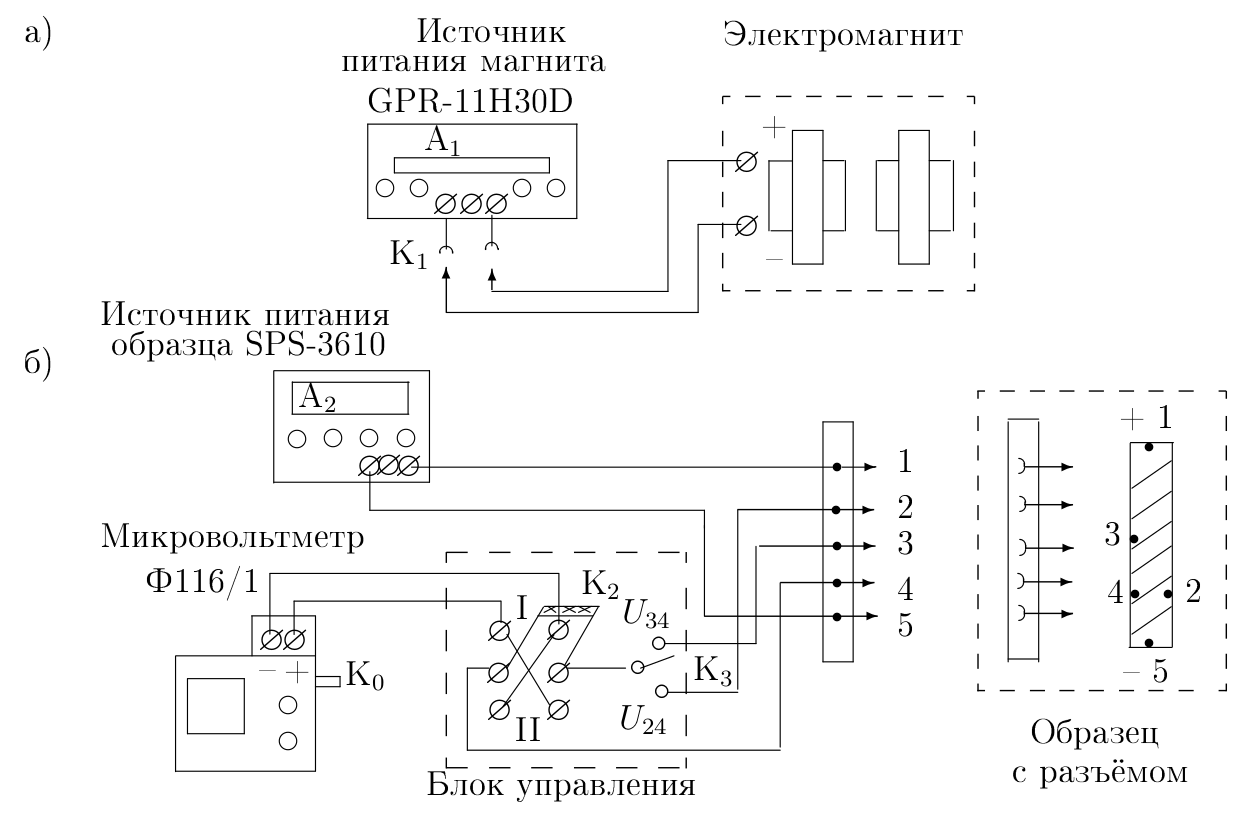
\includegraphics[scale = 0.4]{Workplace}
%     \caption{} \label{work}
% \end{figure}

\parag {Ход работы} ~\\

\point 

\end{document}

